\documentclass[tikz,border=8pt]{standalone}
\usepackage[utf8]{inputenc}
\usepackage[T1]{fontenc}
\usepackage{lmodern}
\usetikzlibrary{arrows.meta,positioning,fit,trees}
\definecolor{navy}{HTML}{15324B}
\definecolor{blue}{HTML}{2F80C1}
\definecolor{cyan}{HTML}{DCEFF7}
\definecolor{orange}{HTML}{E8873A}
\definecolor{green}{HTML}{3B8F72}
\tikzset{box/.style={draw=navy,rounded corners,very thick,align=center,minimum height=1cm,fill=white,font=\sffamily},arr/.style={-{Latex[length=3mm]},very thick,navy}}
\begin{document}
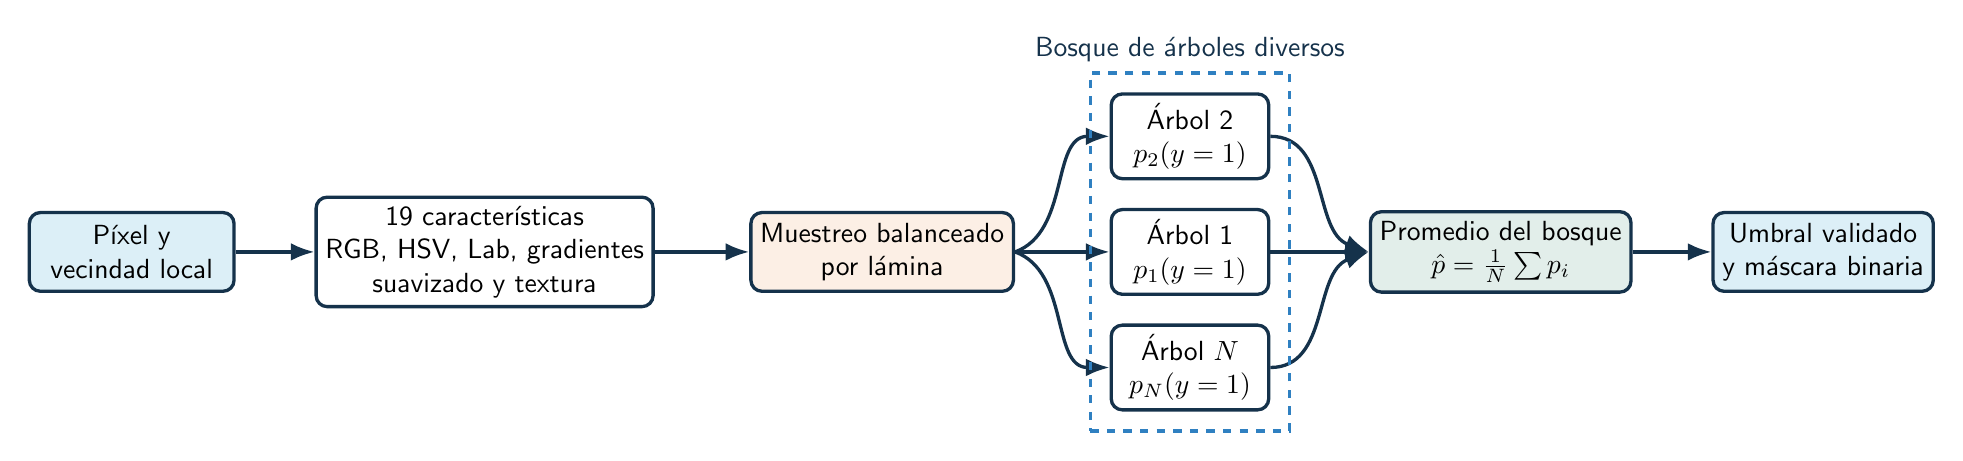
\begin{tikzpicture}[node distance=0.8cm and 1cm]
\node[box,fill=cyan,minimum width=2.6cm] (pixel) {Píxel y\\vecindad local};
\node[box,right=of pixel,minimum width=3.3cm] (features) {19 características\\RGB, HSV, Lab, gradientes\\suavizado y textura};
\node[box,right=1.2cm of features,fill=orange!13,minimum width=2.5cm] (sample) {Muestreo balanceado\\por lámina};
\draw[arr] (pixel)--(features); \draw[arr] (features)--(sample);
\node[box,right=1.2cm of sample,minimum width=2.0cm] (t1) {Árbol 1\\$p_1(y=1)$};
\node[box,above=0.35cm of t1,minimum width=2.0cm] (t2) {Árbol 2\\$p_2(y=1)$};
\node[box,below=0.35cm of t1,minimum width=2.0cm] (tn) {Árbol $N$\\$p_N(y=1)$};
\draw[arr] (sample)--(t1); \draw[arr] (sample.east) to[out=20,in=180] (t2.west); \draw[arr] (sample.east) to[out=-20,in=180] (tn.west);
\node[box,right=1.25cm of t1,fill=green!15,minimum width=2.5cm] (vote) {Promedio del bosque\\$\hat p=\frac{1}{N}\sum p_i$};
\draw[arr] (t1)--(vote); \draw[arr] (t2.east) to[out=0,in=160] (vote.west); \draw[arr] (tn.east) to[out=0,in=200] (vote.west);
\node[box,right=of vote,fill=cyan,minimum width=2.5cm] (mask) {Umbral validado\\y máscara binaria};
\draw[arr] (vote)--(mask);
\node[draw=blue,dashed,very thick,fit=(t1)(t2)(tn),inner sep=7pt,label={[navy,font=\sffamily]above:Bosque de árboles diversos}] {};
\end{tikzpicture}
\end{document}
